\subsubsection{\stid{1.09} Distributed Tasking at Exascale: PaRSEC}


\paragraph{Overview}

The PaRSEC Environment provides a runtime component to dynamically execute on
heterogeneous distributed systems, and a productivity toolbox that comprises a
development framework for the support of multiple domain specific languages
(DSLs) and extensions, with debugging, trace collection, and analysis tools.
%
The PaRSEC project team is dedicated to solving two challenging and
interdependent problems facing the ECP developer community: First, how we create
an execution model that enables developers to express as much parallelism as
possible in their applications, so that those applications effectively utilize
the massive collection of heterogeneous devices that ECP machines will deploy.
Second, how we ensure that that execution model is flexible and portable enough
to actually increase the scientific productivity of those same application
developers, not only for the ECP target environments but for the foreseeable
future.
\begin{wrapfigure}{l}{.6\linewidth}
  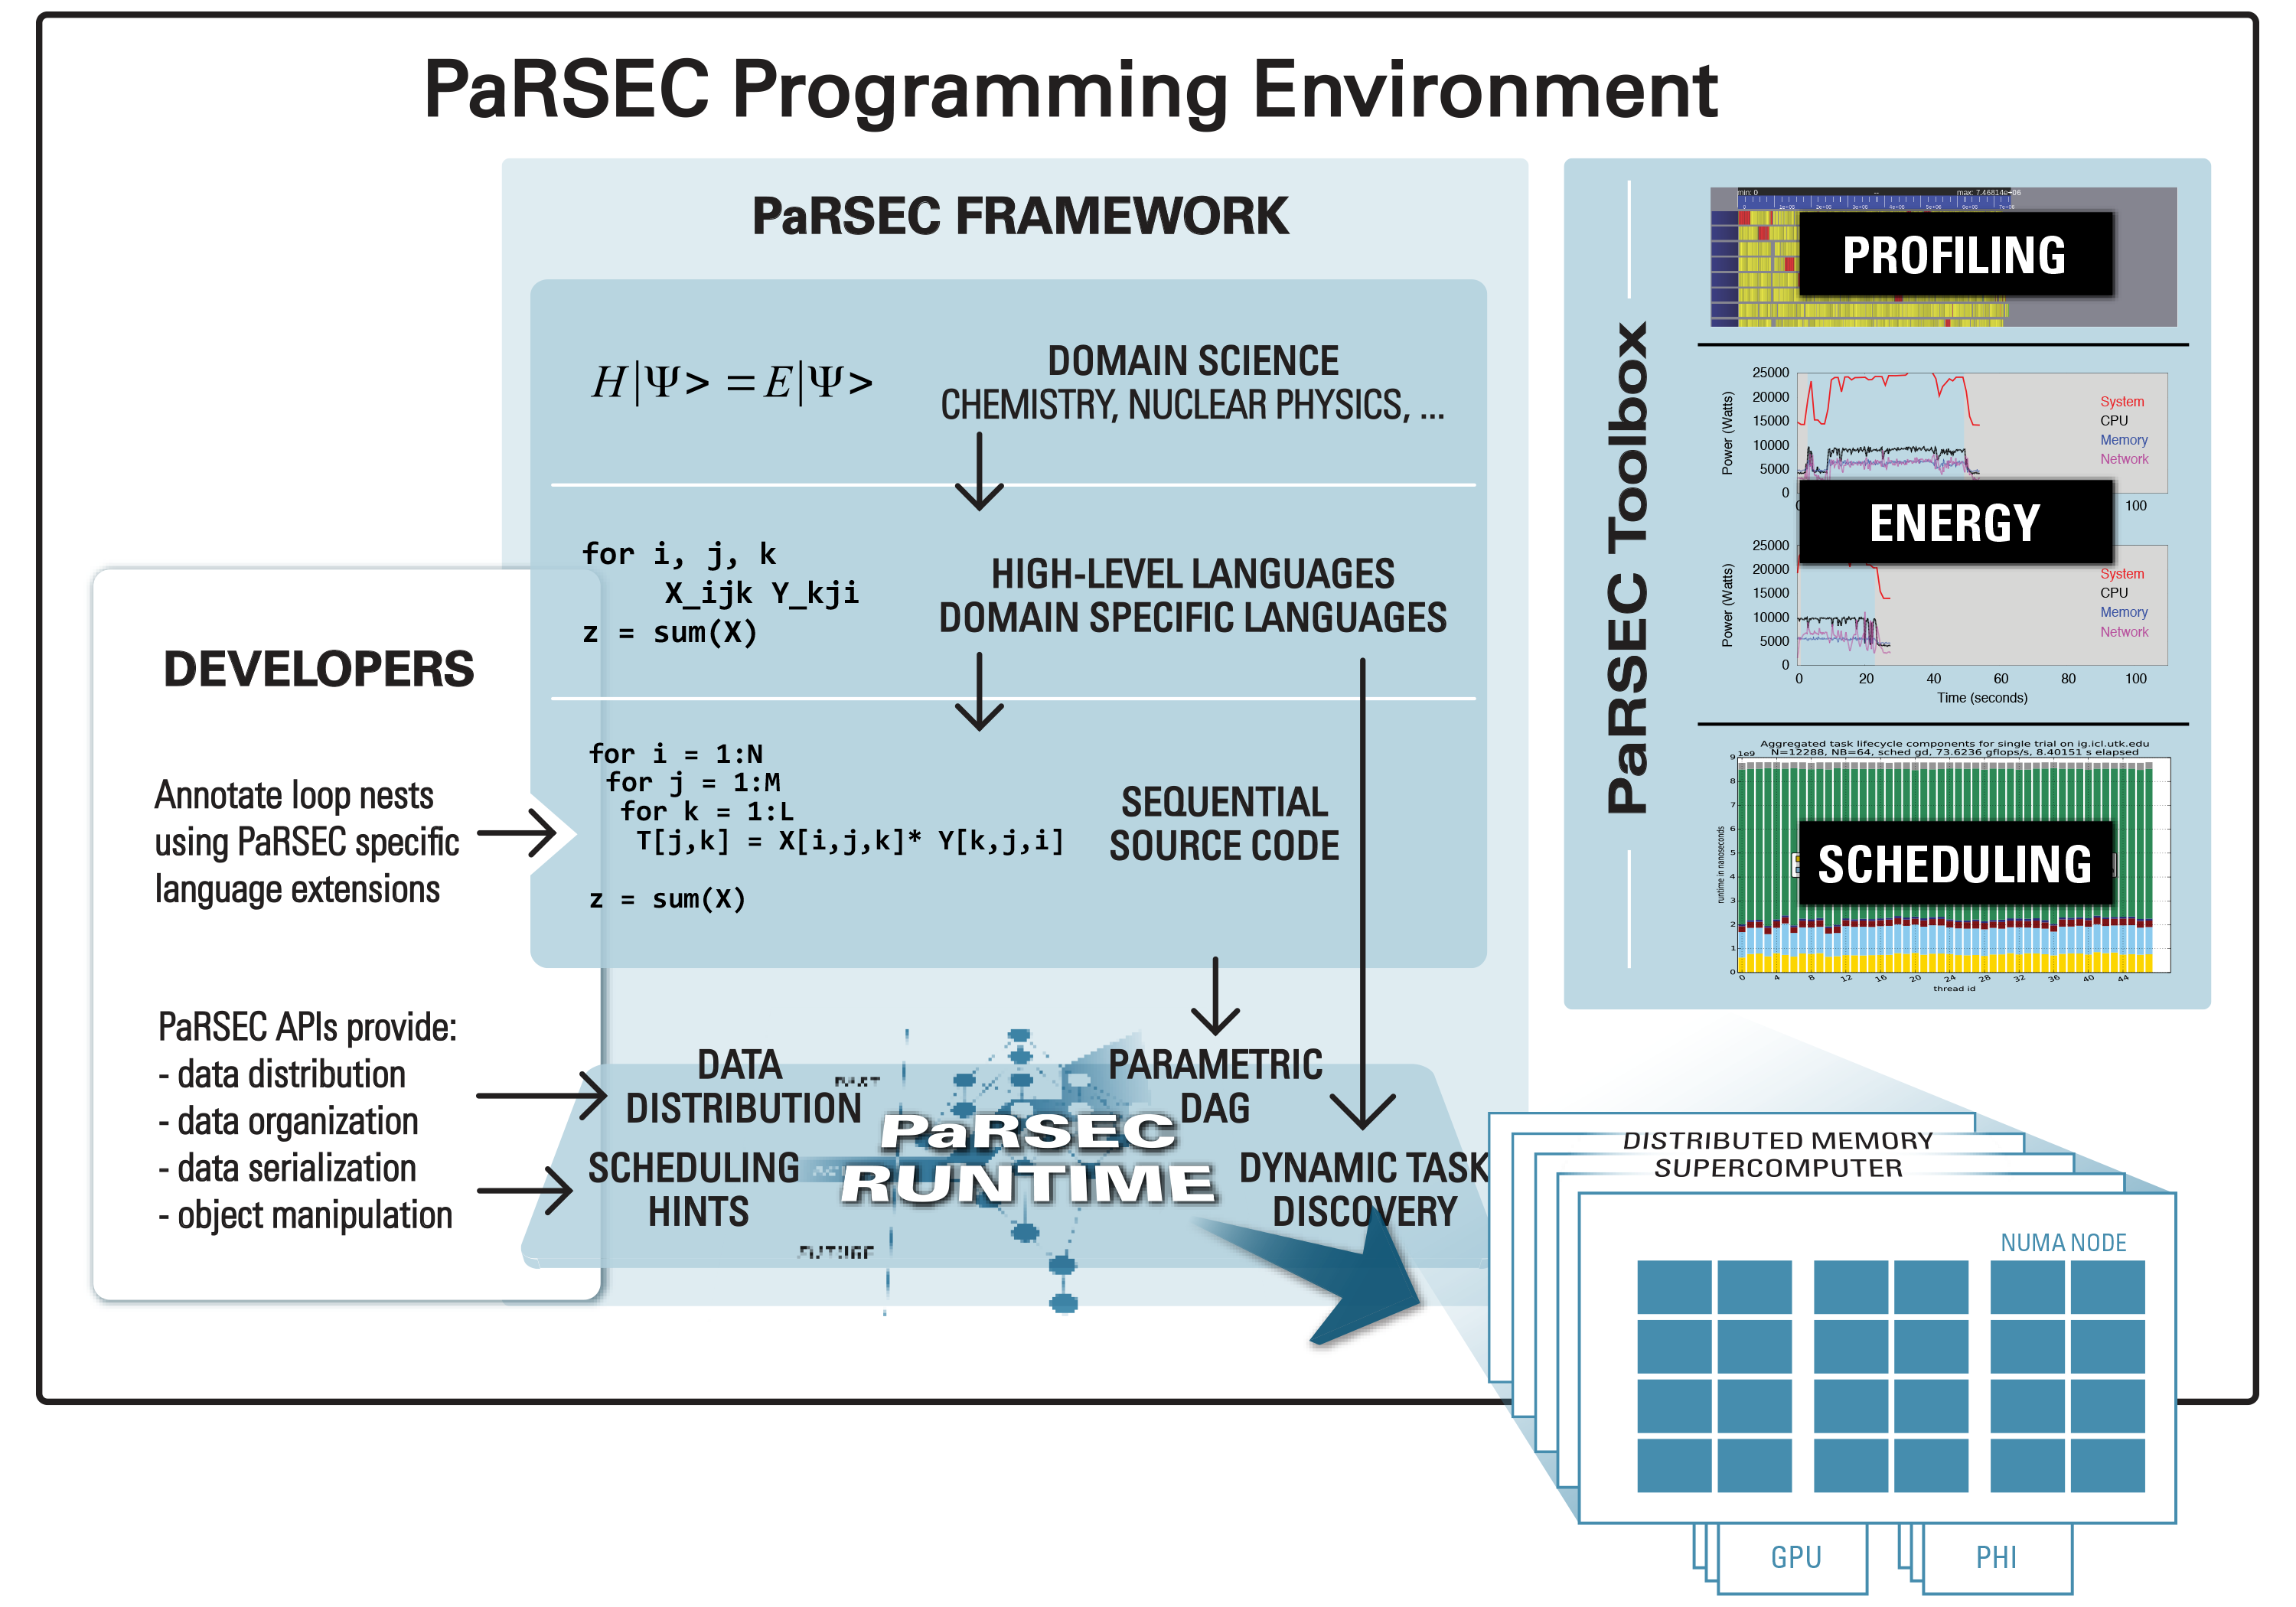
\includegraphics[scale=0.35]{projects/2.3.1-PMR/2.3.1.09-ParSEC/PaRSEC-diagram.png}
  \caption{PaRSEC architecture\label{fig:parsec}}
\end{wrapfigure}
%
PaRSEC is an open source, community-based implementation of a generic task-based
runtime that is freely available, and used by an increasing number of software
libraries.
%  The PARSEC development team is mainly comprised of research staff at % UTK,
%  but regular contributions from the community are provided via our presence %
%  on GitHub and Bitbucket.
The project focuses on prototyping different approaches to define task-based
languages that will be able to exploit the full range of capabilities of
Exascale platforms. Without such a project, and based on the current state of
task-based runtimes, potential users will be stuck either in fixed programming
boundaries, or with particular programming languages. The DTE project provides
means to maintain a high competitiveness in the field leading to more innovation
on addressing the challenges we are facing toward scalable, performant and
Exascale ready programming paradigms.

\paragraph{Key  Challenges}
%\textit{Describe what is hard to do, why it is challenging.}

As we approach Exascale, a number of aspects of the hardware and software
environment pose challenges. First and foremost, keeping pace with the
architectural changes on current and future machines requires changes not only
on how we take advantage of the hardware capabilities, but how we reshape our
algorithms and applications to expose enough parallelism to maximize the use of
the underlying hardware. The number of nodes, threads per node, memory
hierarchies and support for increased computational capabilities (accelerators)
will continue to increase, while the currently available programming paradigms
are still struggling with parallelism at the node level.

\paragraph{Solution Strategy}
%\textit{Describe your basic strategy for addressing the challenges.}
The approach followed in PaRSEC is to provide a low-level, flexible and dynamic
runtime able not only to schedule tasks at the node level, but to handle data
transfers between different memory (both inter and intra nodes), memory
hierarchies, heterogeneous architectures with support for accelerators with a
simple programming scheme. The proposed approach envisions a middle-ground
solution, addressing both hardware and software challenges. At the hardware
level a team of dedicated developers extends PaRSEC to map it's capabilities to
the hardware and to improve it's scalability and performance. At the upper level
the interaction with the users is through building Domain Specific Languages
with the target domain scientists in mind, that will facilitate the expression
of algorithmic parallelism with familiar constructs mapped on the exposed
low-level capabilities. To facilitate the integration of PaRSEC-driven libraries
into larger and complex applications, PaRSEC natively interoperate with other
programming paradigms, including some target of the ECP PMR support, such as
PGAS, MPI, OpenMP and Kokkos. This integration provides a smooth transition for
library developers that embrace the PaRSEC runtime, providing a platform where a
shift to a new programming paradigms can be done in stages of increased
complexity.
% In this model, PaRSEC remains in full control of data tracking and
% allocation on the managed accelerator.

\paragraph{Recent Progress}

\begin{wrapfigure}{l}{.45\linewidth}
  \centering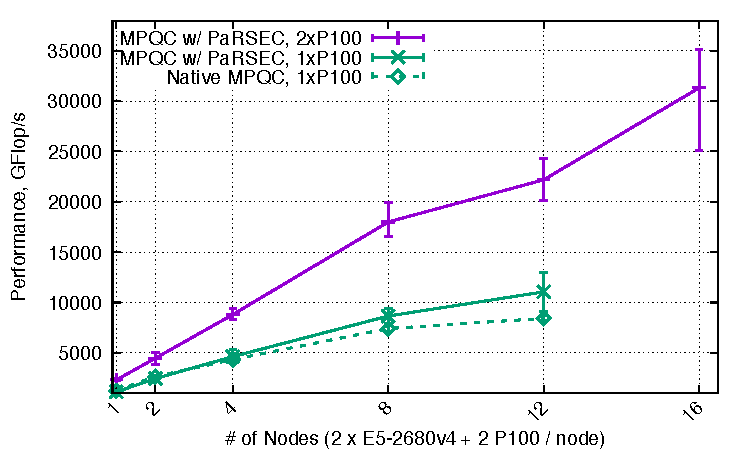
\includegraphics[scale=0.55]{projects/2.3.1-PMR/2.3.1.09-ParSEC/cc_abcd.pdf}
  \caption{Strong-scaling performance of the ABCD term in the coupled-cluster doubles equation for $(H_2O)_{12}$ in aug-cc-pVDZ basis set.\label{fig:MPQC}}
\end{wrapfigure}
The DTE GPU support engine has been refactored, enabling unprecedented
performance on distributed, multi-GPU platforms for real applications,
like MPQC, which is part of the NWChemEx chemistry
package. Figure~\ref{fig:MPQC} shows a strong scaling performance of
MPQC using PaRSEC to power the most compute intensive operation of the
tensor contraction, and compares it with native MPQC. This
integration illustrates inter-runtimes cooperation, as the
vast majority of MPQC remains supported by its current runtime
system, and only a tensor contraction, runs over
the PaRSEC runtime.
% Both runtime systems thus collaborate to the general progress of the application.
The refactoring of the GPU engine in PaRSEC, and the task system programming
approach, however, allow to support multiple GPUs without code modification,
while the native MPQC implementation does not. PaRSEC supported DTE shows an
efficient strong scaling, even with multiple accelerators.

An important aspect of the DTE project is to define and prototype scalable
domain specific languages that enable a productive expression of parallelism for
end-user communities. PaRSEC presents multiple programming interfaces
(Parameterized Task Graphs for maximum parallelism, the popular serial task
insertion dataflow model to provide direct access to the runtime). In addition
the DTE team is in close contact with application teams to define parallel
abstractions that are suitable for their domain usage. Notably, the PaRSEC team
has ongoing collaboration with the SLATE linear algebra package and NWChemEx
chemistry package teams.
The PaRSEC development team did the first step toward the integration
of their framework into the SLATE (2.3.3.09) in the context of the
shared milestone (STPM11-23). The first prototype of the application
ran in a distributed environment and showed the capability of the
SLATE library using a modern fully capable runtime system. This work
involved enhancing the insert task interface available in the ParSEC
runtime to map onto the logic of a SLATE algorithm.

\begin{wrapfigure}[16]{l}{.45\linewidth}
  \vspace*{-1em}\centering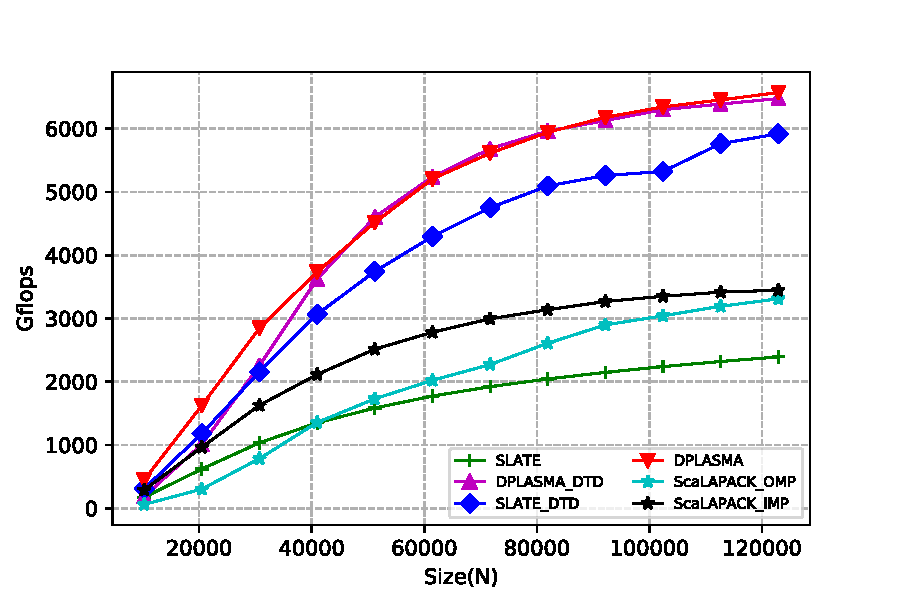
\includegraphics[scale=0.55]{projects/2.3.1-PMR/2.3.1.09-ParSEC/SLATE_inital_result_phicluster_scalapack.pdf}
  \caption{Comparison of DPLASMA and SLATE Cholesky factorization over PaRSEC with
           SLATE and ScaLAPACK on 64 nodes 12 cores each\label{fig:slate-parsec}}
\end{wrapfigure}
%
In figure~\ref{fig:slate-parsec}, we compare the integration of SLATE
and PaRSEC against the state of the art. First against the two legacy
domain specific languages that have the capability to do linear
algebra; then against the regular SLATE using OpenMP for intra-node
parallelism, and MPI for communication; and finally against ScaLAPACK,
which is the reference for distributed linear algebra.

On the software quality side, the PaRSEC runtime has been evaluated and amended
to compile and run on all major target pre-Exascale platforms (ALCF Mira, Theta; OLCF
Titan, Summit-dev). In particular the detection of architecture specific
features on NVIDIA V100 accelerators and Power processors has been improved.
PaRSEC now includes a Spack definition file to ease the deployment on future
target systems as part of the system software SDK effort.

\paragraph{Next Steps}
%\textit{Describe what you are working on next.}
% Improve DTE accelerator support and interoperability with other
% programming models
To provide programmers with more supervision over how accelerators are
integrated and used by the runtime, a need to provide finer control of the
resource usage by the runtime system has arisen. We are developing new APIs to
allow the programmers to advise the runtime system with respect to data
placement, prefetching, and management of cache.
%
Programming interoperability should not be limited to node-level programming
models but should extend to distributed programming. Execution modes where part
of the application is expressed in native MPI (including communicating tasks)
and other parts using PaRSEC DSLs, running above the task system in a tightly
coupled manner, are being developed.

% Facilitate DSL integration

% Provide better libraries and tools integration
The set of tools that come with the PaRSEC runtime environment to
assess performance, find bottlenecks, improve scheduling and debug the
task-based application are being improved to expose the information
in a format compatible with TAU, Score-P and other
tools that are already familiar to ECP users.
